
On-Policy Distillation (OPD) has established itself as a cornerstone of the modern post-training pipeline for Large Language Models (LLMs). By aligning a student model with a superior teacher through trajectories sampled from its own policy, OPD enables a token level of reasoning refinement that goes beyond static Supervised Fine-Tuning (SFT). This effectiveness has been validated by industrial works such as DeepSeek-V4~\cite{deepseekv4}, MiMo~\cite{xiao2026mimo}, and Qwen-3~\cite{qwen3technicalreport}, where OPD serves as a vital component alongside SFT or Reinforcement Learning with Verifiable Rewards (RLVR) to further squeeze out reasoning performance.


% In existing OPD research, high-loss tokens are generally characterized as potential "critical branching points" where the student's policy deviates significantly from the teacher's trajectory, thus serving as the primary drivers of policy correction~\cite{lu2025onpolicydistillation}. Intuitively, as the student aligns with the teacher during the OPD process, both the magnitude and cardinality of these high-loss tokens are expected to diminish, eventually leading to an optimization plateau. However, our empirical investigations reveal a striking phenomenon: even after training has reached apparent saturation, a stubborn population of tokens—which we formally define as \textbf{Rock Tokens}—continues to exhibit consistently high loss. Notably, while these tokens represent a small minority of the vocabulary (approximately 6\%), they account for as much as 50\% of the total token frequency in the model's output. This persistence challenges conventional understanding of model convergence and raises a fundamental question: \textit{Are Rock Tokens indispensable Pillars for policy alignment, or are they Stumbling Blocks that create unnecessary optimization redundancy?}

Recent studies in Reinforcement Learning with Verifiable Rewards (RLVR) have revealed that not all tokens contribute equally to model learning: a small subset of critical tokens, such as high-entropy "forking tokens" at decisive branching points, disproportionately drives reasoning gains~\cite{wang2025beyond}. While this token-level perspective has reshaped our understanding of RLVR dynamics, an analogous investigation in OPD remains largely unexplored, despite OPD's reliance on dense token-level supervision. In this work, we initiate such an investigation by focusing on a token type uniquely meaningful to the OPD paradigm: high-loss tokens. Unlike RLVR, where token importance is inferred from policy entropy or reward signals, OPD provides a direct measure of student-teacher mismatch through per-token KL divergence; high-loss tokens thus explicitly mark the positions where the student's policy diverges most sharply from the teacher's, making them natural candidates for the ``critical correction points'' that drive alignment~\cite{lu2025onpolicydistillation}. 

Intuitively, as the student aligns with the teacher during the OPD process, both the magnitude and cardinality of these high-loss tokens are expected to diminish, eventually leading to an optimization plateau. However, our empirical investigations reveal a striking phenomenon: even after training has reached apparent saturation, a stubborn population of tokens—which we formally define as Rock Tokens—continues to exhibit consistently high loss. Notably, while these tokens represent a small minority of the vocabulary (approximately 6\%), they account for as much as 50\% of the total token frequency in the model's output. This persistence challenges conventional understanding of model convergence and raises a fundamental question: Are Rock Tokens indispensable Pillars for policy alignment, or are they Stumbling Blocks that create unnecessary optimization redundancy?


\begin{figure}[t]
  \centering
  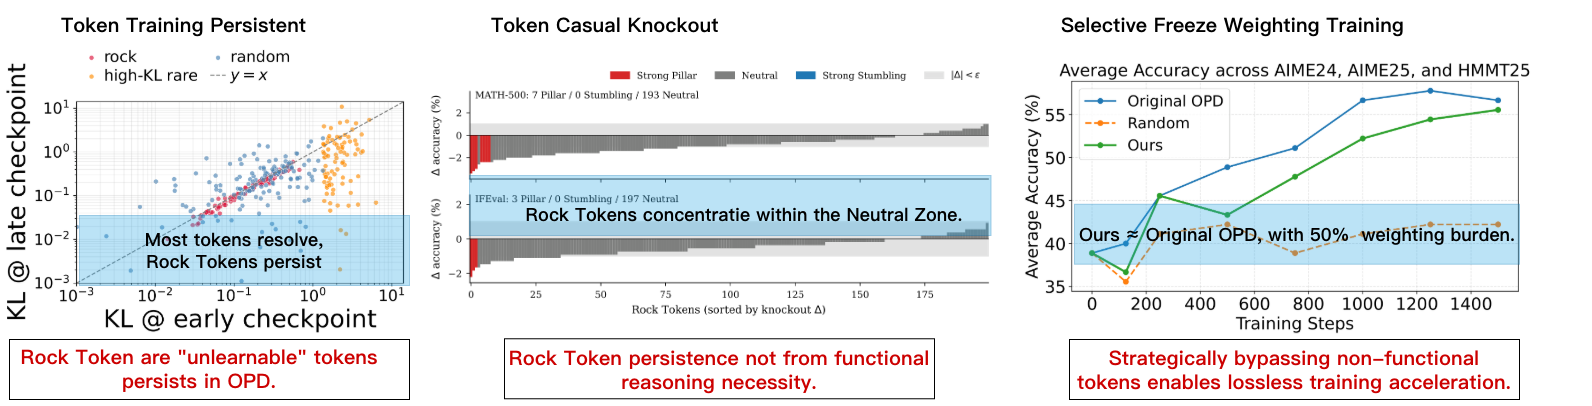
\includegraphics[width=\linewidth]{Figures/rock_intro.png}
  \caption{\textbf{The lifecycle and functional impact of Rock Tokens in OPD.} (a) \textbf{Phenomenon}: Identification of optimization-resistant tokens. (b) \textbf{Mechanism}: Causal evidence of structural redundancy via token knock-out. (c) \textbf{Utility}: Performance parity achieved through strategic gradient sparsification.}
  \label{fig:intro}
\end{figure}



To provide a systematic understanding of the Rock Token phenomenon, our research is structured across three investigative dimensions: identifying \textbf{what} are rock tokens, analyzing \textbf{why} they emerge and persist, and uncovering \textbf{how} they collectively impact the overall OPD training process. This comprehensive framework is operationalized through the following three stages:

First, we characterize the identity of Rock Tokens (What). We begin by identifying Rock Tokens linguistic and statistical properties, revealing that they primarily comprise \textbf{syntactic and structural scaffolding}—such as formatting delimiters, whitespace symbols, and high-frequency discourse markers (e.g., ``So'', ``Wait''). To determine the dynamic role of these elements, we employ quantitative gradient dynamics analysis to address \textbf{RQ1: Do Rock Tokens still provide useful learning signals during optimization?} By examining whether their persistent high loss effectively translates into constructive gradients, we assess whether these tokens offer steady directional guidance or merely represent stagnant optimization noise throughout the OPD process.

Second, we investigate the underlying mechanisms behind their persistence (Why). Beyond the actual contribution of Rock Tokens during training is clarified, a more profound question emerges: \textbf{why do these tokens persist in the first place?} We hypothesize that the student model develops a strong decoding dependency on these specific tokens to maintain its reasoning flow, creating a path dependency that resists corrections from the teacher model. This leads to our \textbf{RQ2: Does Rock Token persistence stem from student path dependency?} To investigate this, we conduct \textit{token knock-out} experiments as a form of ablation analysis, examining whether the student's logical coherence is so deeply intertwined with these persistent residuals that it becomes structurally unable to shift its policy toward the teacher's distribution.

Finally, we evaluate how Rock Tokens influence the overall OPD training process (How). Finally, we arrive at a provocative question: what would happen if these tokens were excluded from the very beginning of OPD training? This leads to our final investigation, \textbf{RQ3: What is the genuine functional contribution of Rock Tokens to model training?} By freezing the gradients of these tokens from the onset of training, we intuitively isolate their functional necessity throughout the entire distillation process. This causal intervention allows us to rigorously determine whether Rock Tokens serve as indispensable pillars of the model's reasoning integrity or if they represent a strategic opportunity to bypass computational redundancy and optimize the efficiency of the alignment pipeline.

In summary, our key contributions are as follows:


\begin{itemize}[leftmargin=*,itemsep=1pt]
    \vspace{-2mm}
    \item For the first time, we identify and characterize \textbf{Rock Tokens}, a persistent high-loss phenomenon that unveils a previously hidden aspect of optimization dynamics in On-Policy Distillation.
    \vspace{-1mm}
    \item We deconstruct the intricate dynamics of the OPD process by systematically uncovering the functional roles of Rock Tokens across both the training and inference phases.
    \vspace{-1mm}
    \item Our research reveals a critical inefficiency in current alignment pipelines, demonstrating that a substantial portion of training signals in OPD provides significantly lower-than-expected contributions to the model's ultimate reasoning performance.
\end{itemize}
